\section{Simulation Study for Inner-loop Controller}
\label{sec:simulation}

It is difficult to evaluate the performance of the control systems in a limited area since changing and holding the quadrotor's attitude makes the quadrotor to move out of our physical test area. Therefore, it is more suitable to use simulation rather than real flight for evaluation of the quadrotor's performance.

The PID inner-loop controller and a linear mapping model from torque into motor speeds described in Section \ref{sec:pid} are often used for attitude control of a quadrotor. Let it be called "linear attitude controller". In this section, simulations of the linear and nonlinear attitude control systems are stated, and comparison of the results is discussed to validate the advantage of the control system stated in Chapter \ref{ch:control_system}. First, setup for simulation is explained., and then, simulation results of the two control systems are discussed.

%%%%%%%%%%%%%%%%%%%%%%%%%%%%%%%%%%%%%%%%%%%%%%%%%%%%%%%%%%%%%%%%%%%%%%%%%%%%%%%%%%%%%%%
\subsection{Simulation Setup}

In simulation, the dynamic models of Equations (\ref{eq:newton_gravity}) and (\ref{eq:rotation}) are applied. The physical quantities of the quadrotor are the same as stated in Chapter \ref{ch:system} in each case. The inner-loop controller was simulated with the following cases; \\
\begin{enumerate}
\item \({\boldsymbol \eta}_d = ({\pi \over{6}}, 0, 0)\)
\item \({\boldsymbol \eta}_d = ({\pi \over{3}}, 0, 0)\)
\item \({\boldsymbol \eta}_d = (0, {\pi \over{6}}, 0)\)
\item \({\boldsymbol \eta}_d = (0, {\pi \over{3}}, 0)\)
\item \({\boldsymbol \eta}_d = (0, 0, {\pi \over{4}})\)
\item \({\boldsymbol \eta}_d = (0, 0, {\pi \over 2})\)
\item \(
\begin{aligned}
{\boldsymbol \eta}_d = 
\begin{cases}
     ({\pi \over{6}}, {\pi \over{6}}, 0) \quad &  1 \le t \le 2 \\
    (-{\pi \over{6}}, -{\pi \over{6}}, 0) \quad & 3 \le t \le 4 \\ 
    (0, 0, 0)  \quad &  \text{otherwise} \\
  \end{cases}
  \end{aligned}
  \)
\end{enumerate}
In every case, the magnitude of thrust control \(F_d\) is constant to be \(mg\), and each controller is well-tuned. 
 
%%%%%%%%%%%%%%%%%%%%%%%%%%%%%%%%%%%%%%%%%%%%%%%%%%%%%%%%%%%%%%%%%%%%%%%%%%%%%%%%%%%%%%%
\subsection{Results}
The results of simulation is shown below. Figure \ref{fig:sim_1} - \ref{fig:sim_7} shows the result of each case in Section \ref{sec:pid}. \\
\begin{figure}[p]
    \centering
    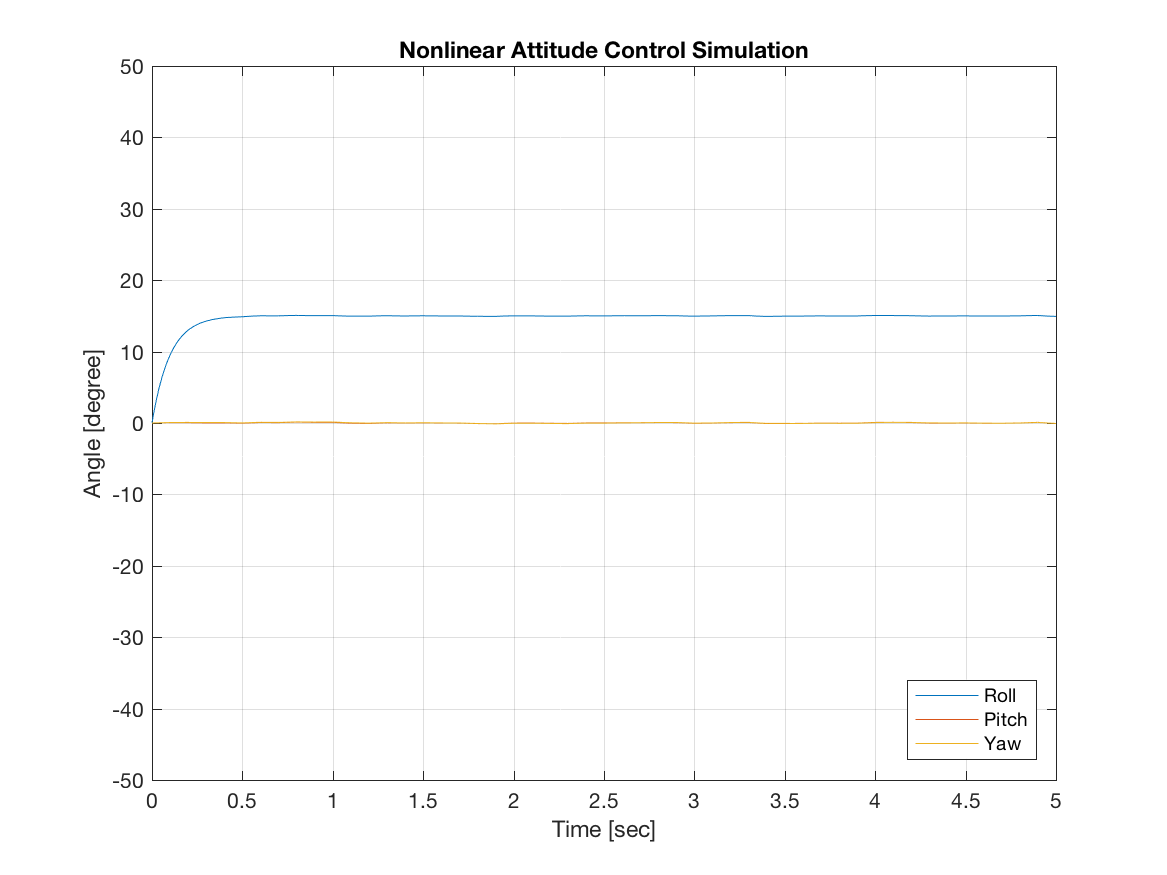
\includegraphics[width=0.45\textwidth]{graphics/phi_03_non.png}
    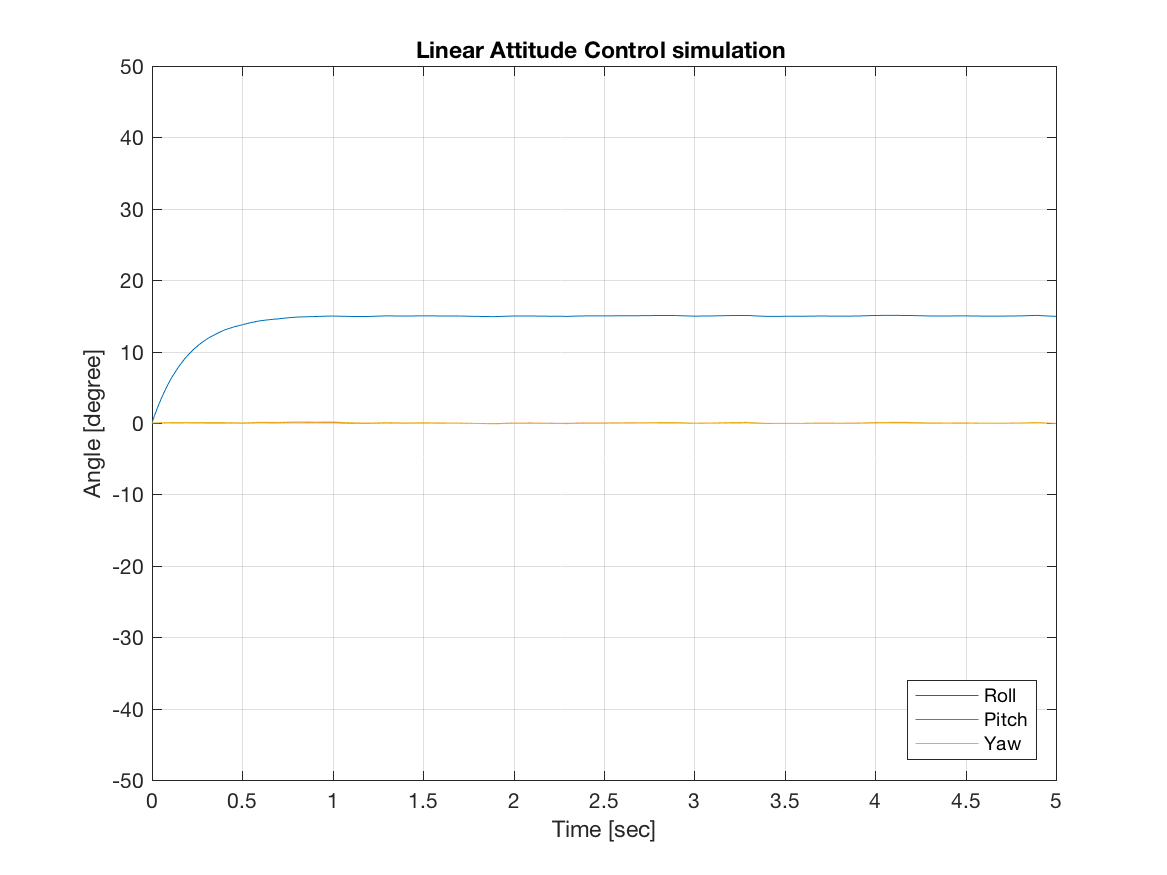
\includegraphics[width=0.45\textwidth]{graphics/phi_03_pid.png}
    \caption{Simulation Result (Case 1)}
    \label{fig:sim_1}
\end{figure}

\begin{figure}
    \centering
    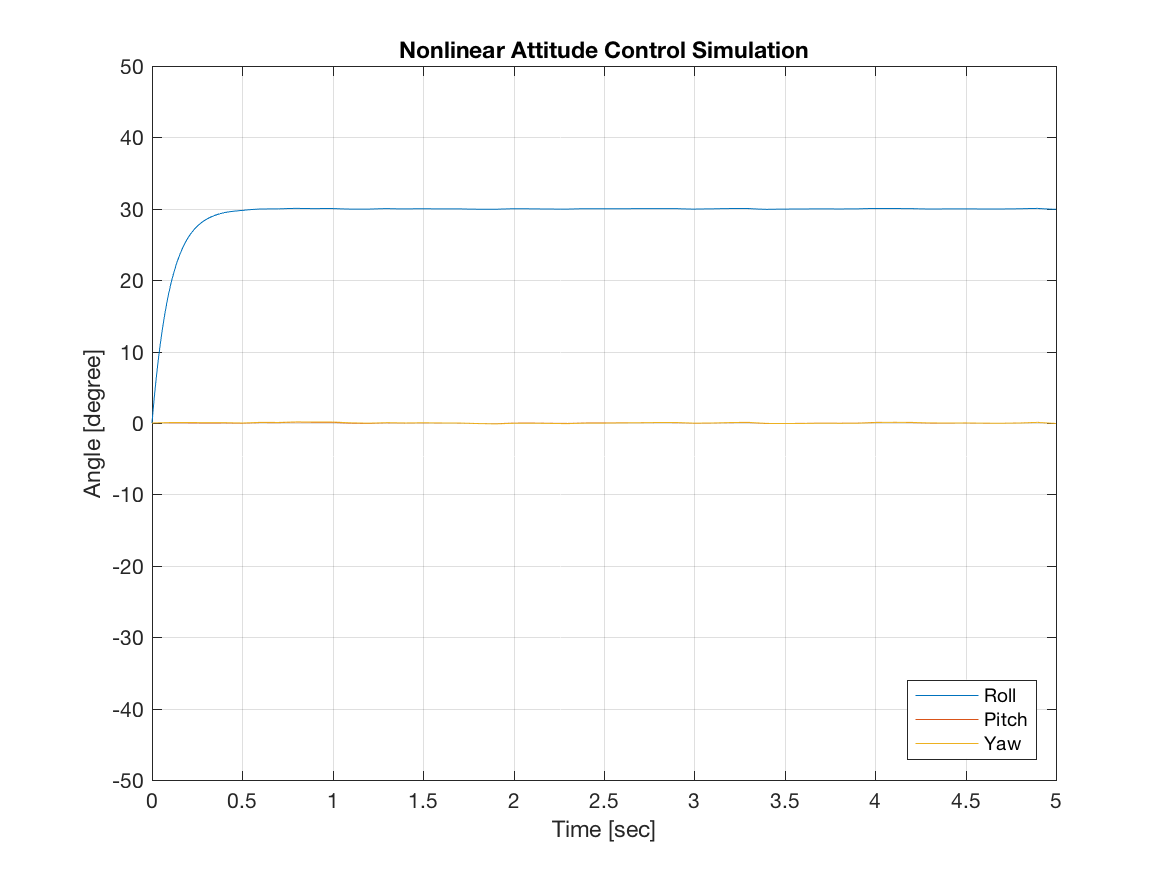
\includegraphics[width=0.45\textwidth]{graphics/phi_05_non.png}
    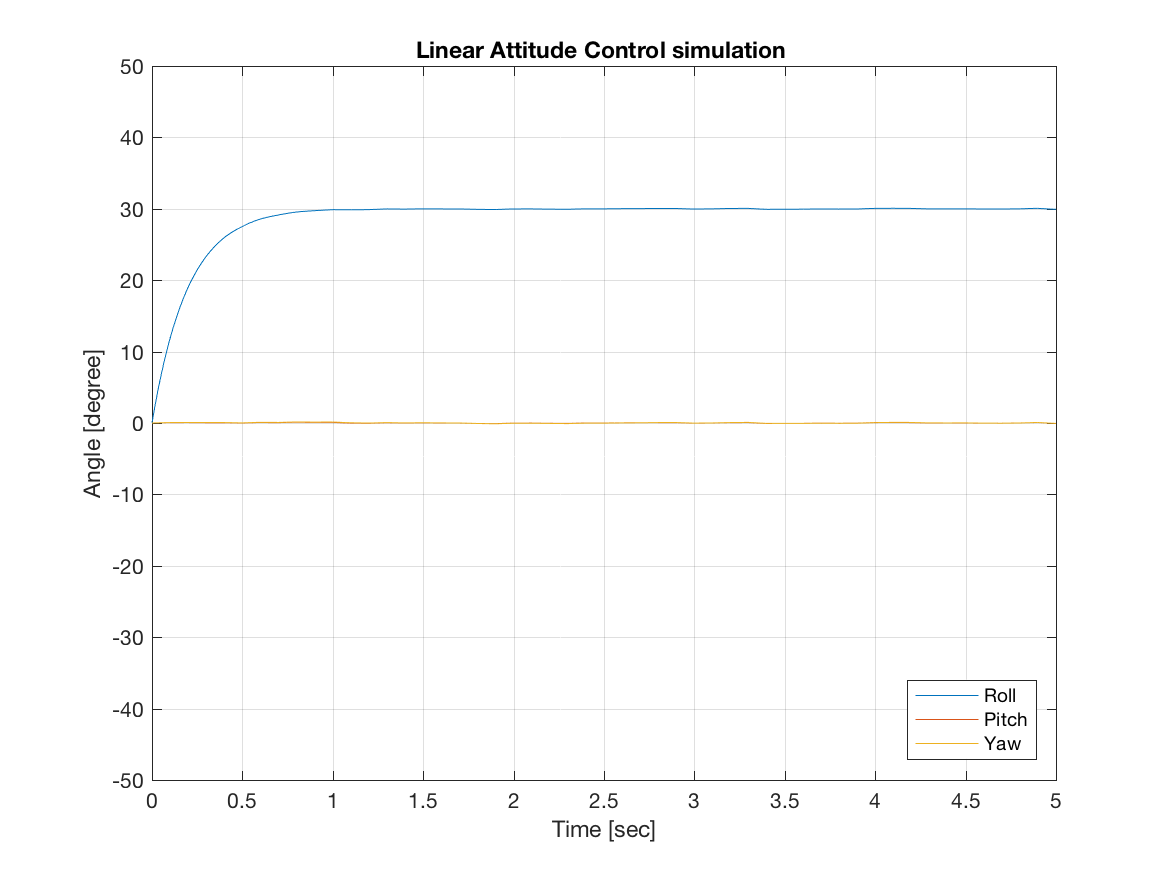
\includegraphics[width=0.45\textwidth]{graphics/phi_05_pid.png}
    \caption{Simulation Result (Case 2)}
    \label{fig:sim_2}
\end{figure}

\begin{figure}
    \centering
    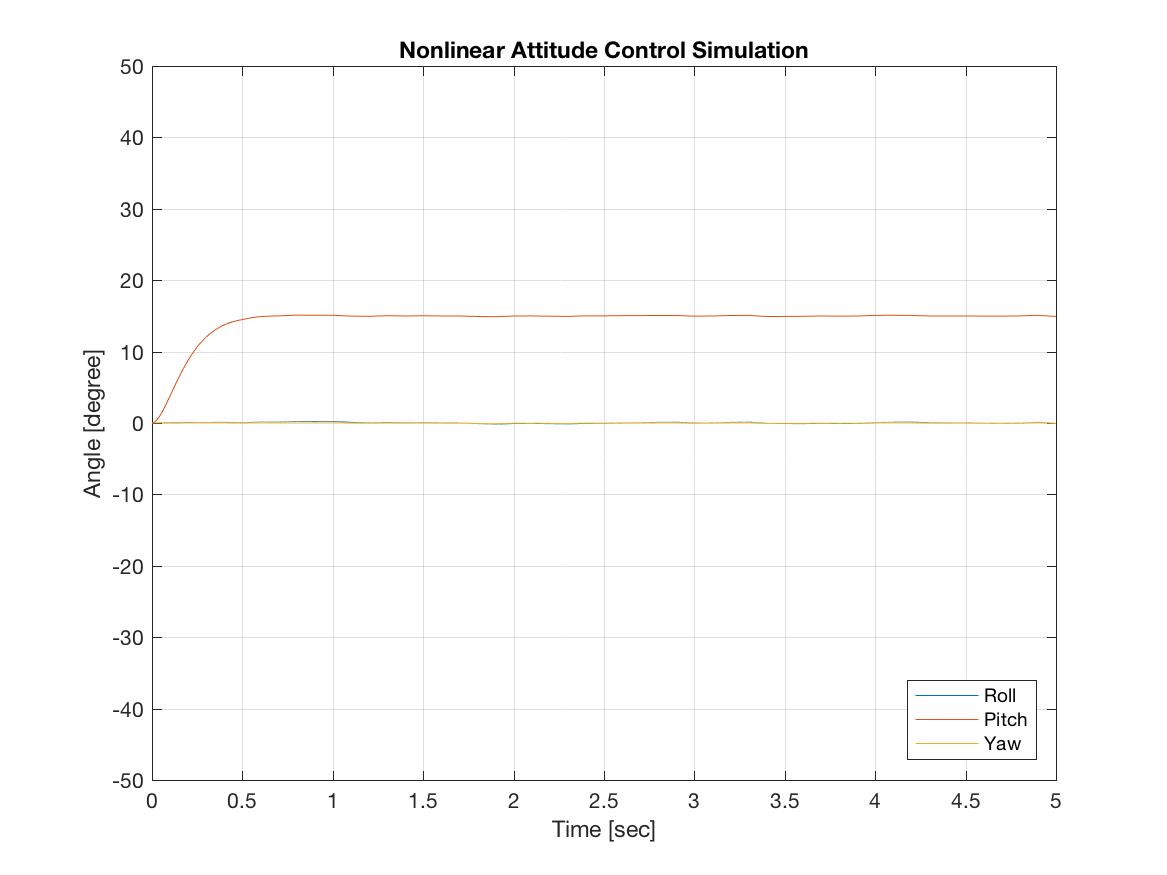
\includegraphics[width=0.45\textwidth]{graphics/theta_03_non.png}
    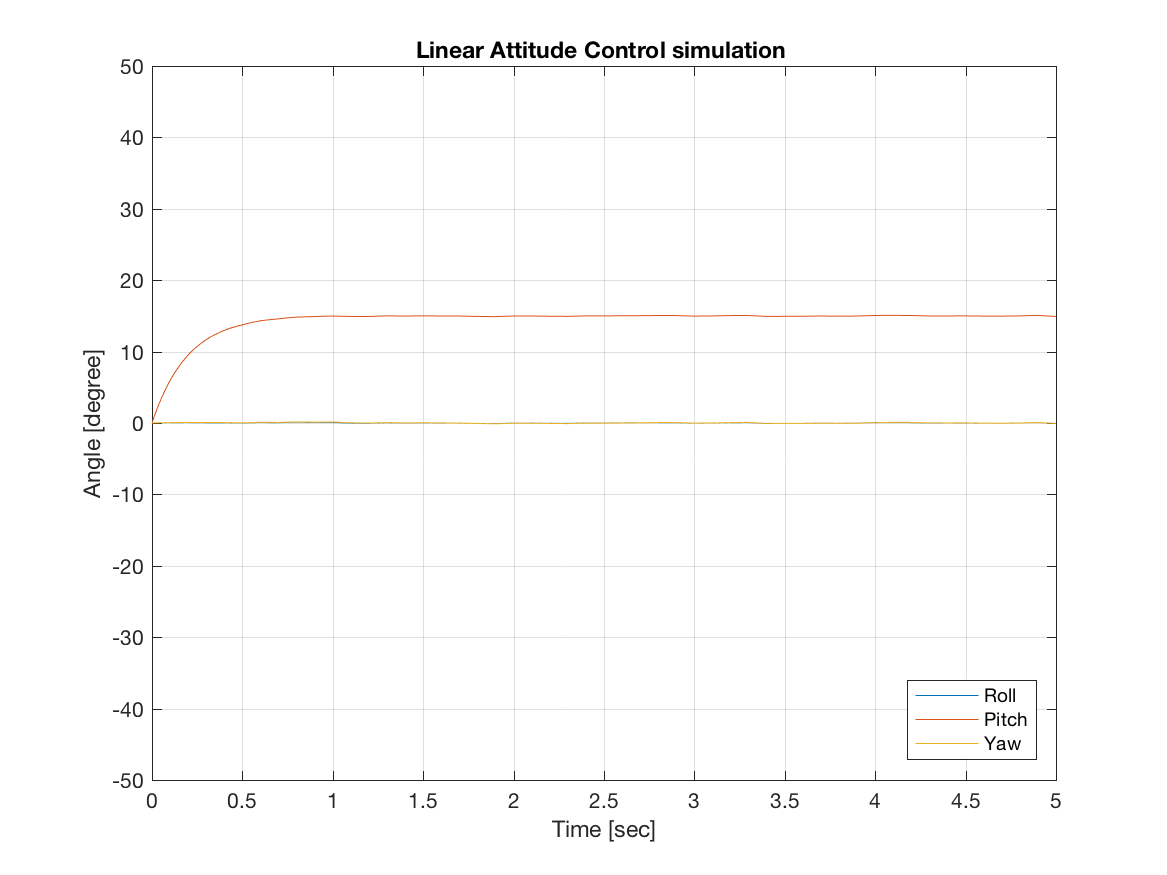
\includegraphics[width=0.45\textwidth]{graphics/theta_03_pid.png}
    \caption{Simulation Result (Case 3)}
    \label{fig:sim_3}
\end{figure}

\begin{figure}
    \centering
    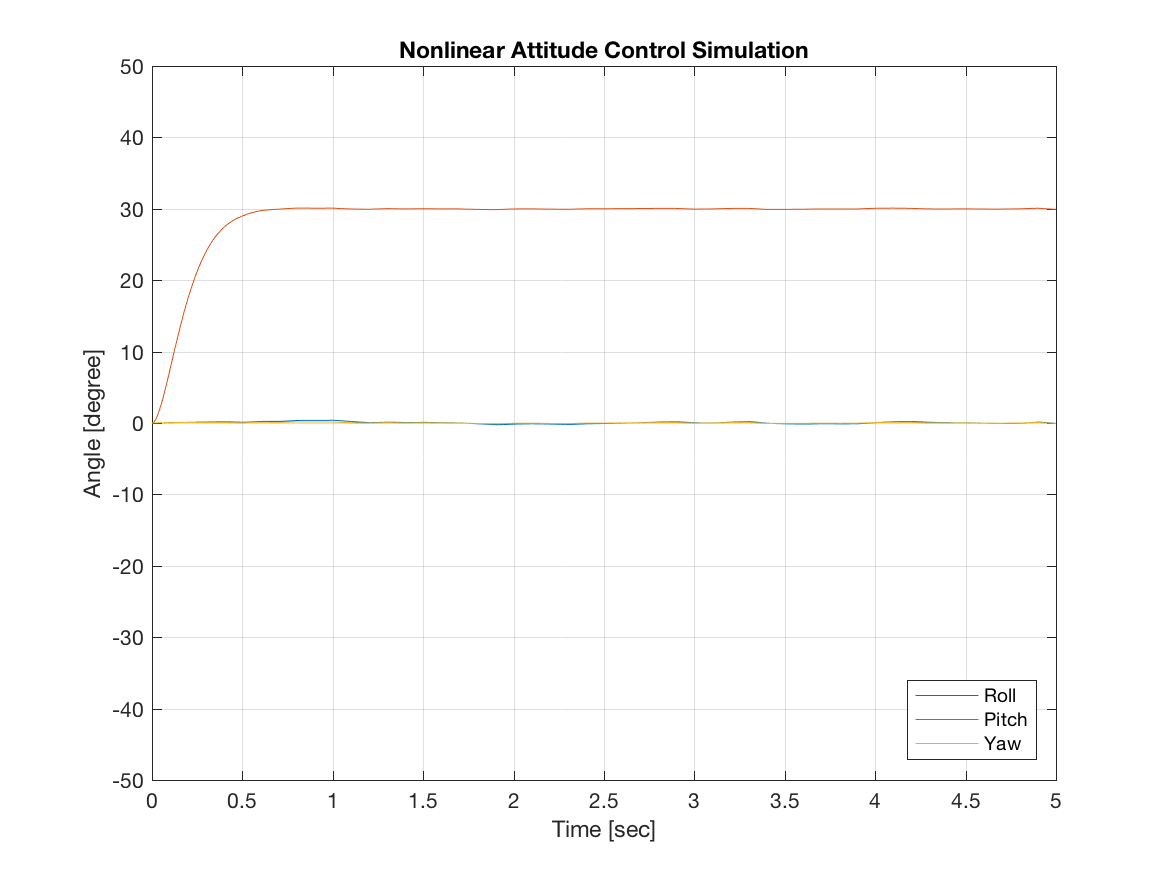
\includegraphics[width=0.45\textwidth]{graphics/theta_05_non.png}
    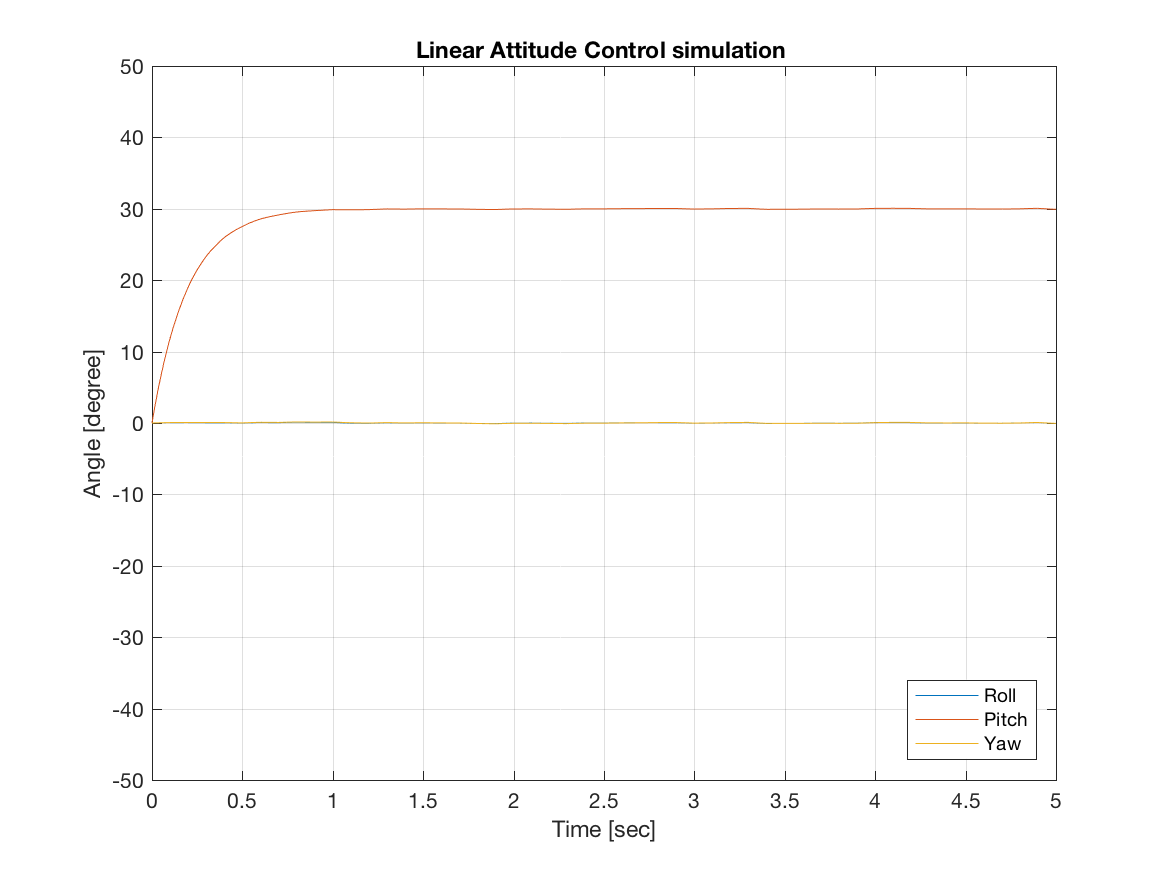
\includegraphics[width=0.45\textwidth]{graphics/theta_05_pid.png}
    \caption{Simulation Result (Case 4)}
    \label{fig:sim_4}
\end{figure}

\begin{figure}
    \centering
    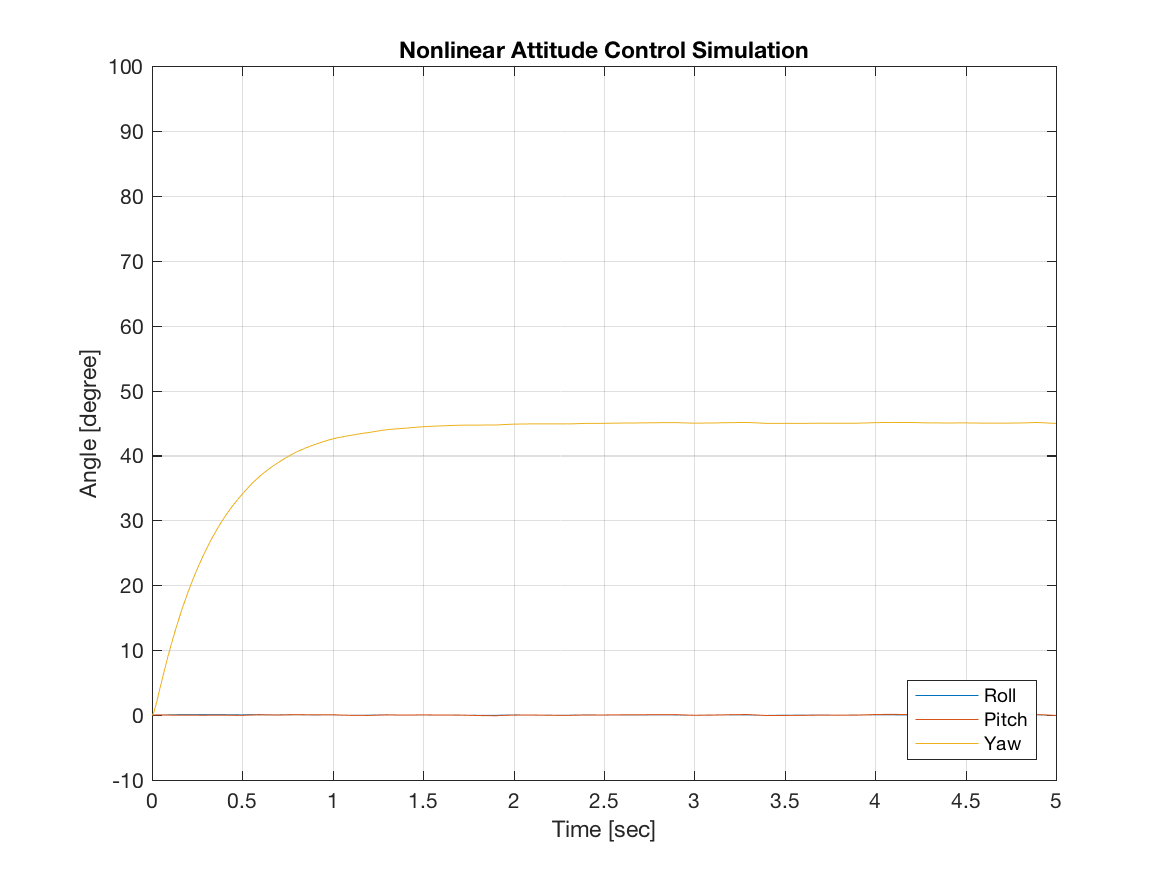
\includegraphics[width=0.45\textwidth]{graphics/yaw_quarter_non.png}
    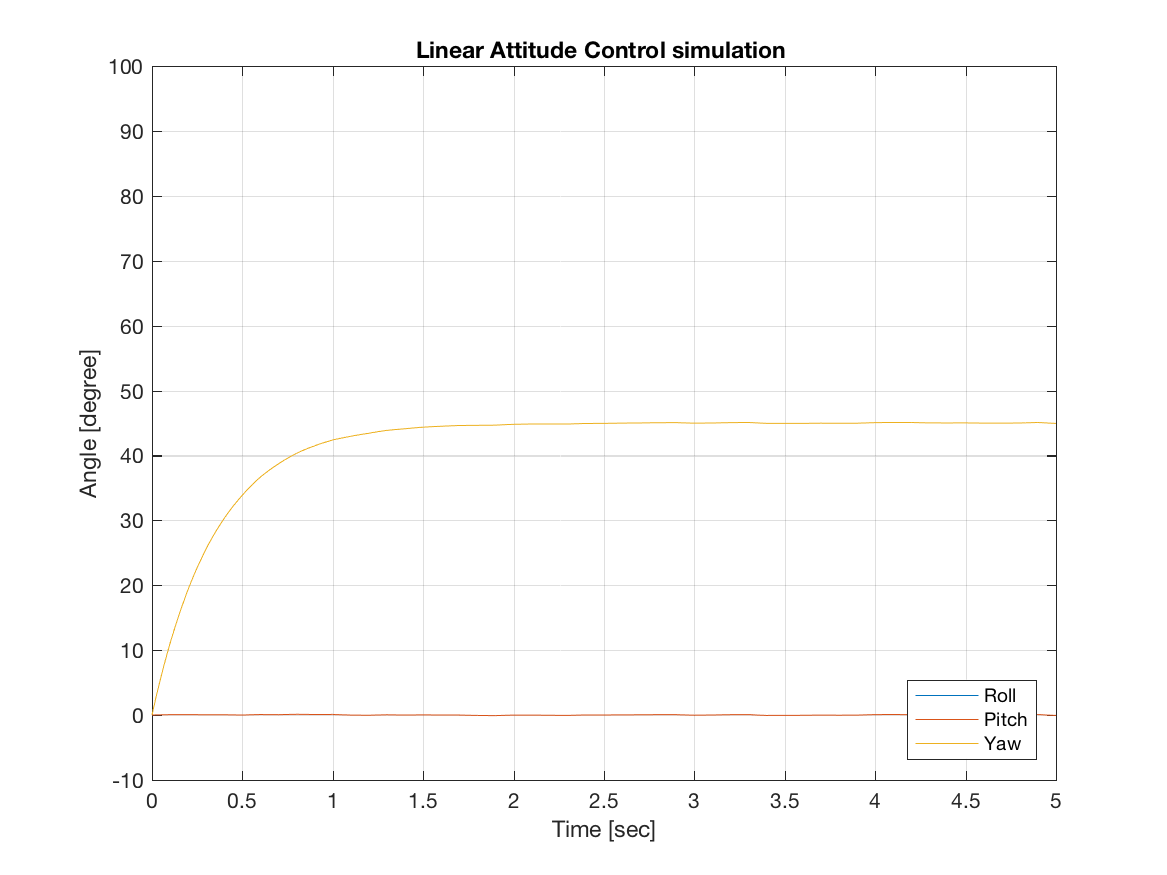
\includegraphics[width=0.45\textwidth]{graphics/yaw_quarter_pid.png}
    \caption{Simulation Result (Case 5)}
    \label{fig:sim_5}
\end{figure}

\begin{figure}
    \centering
    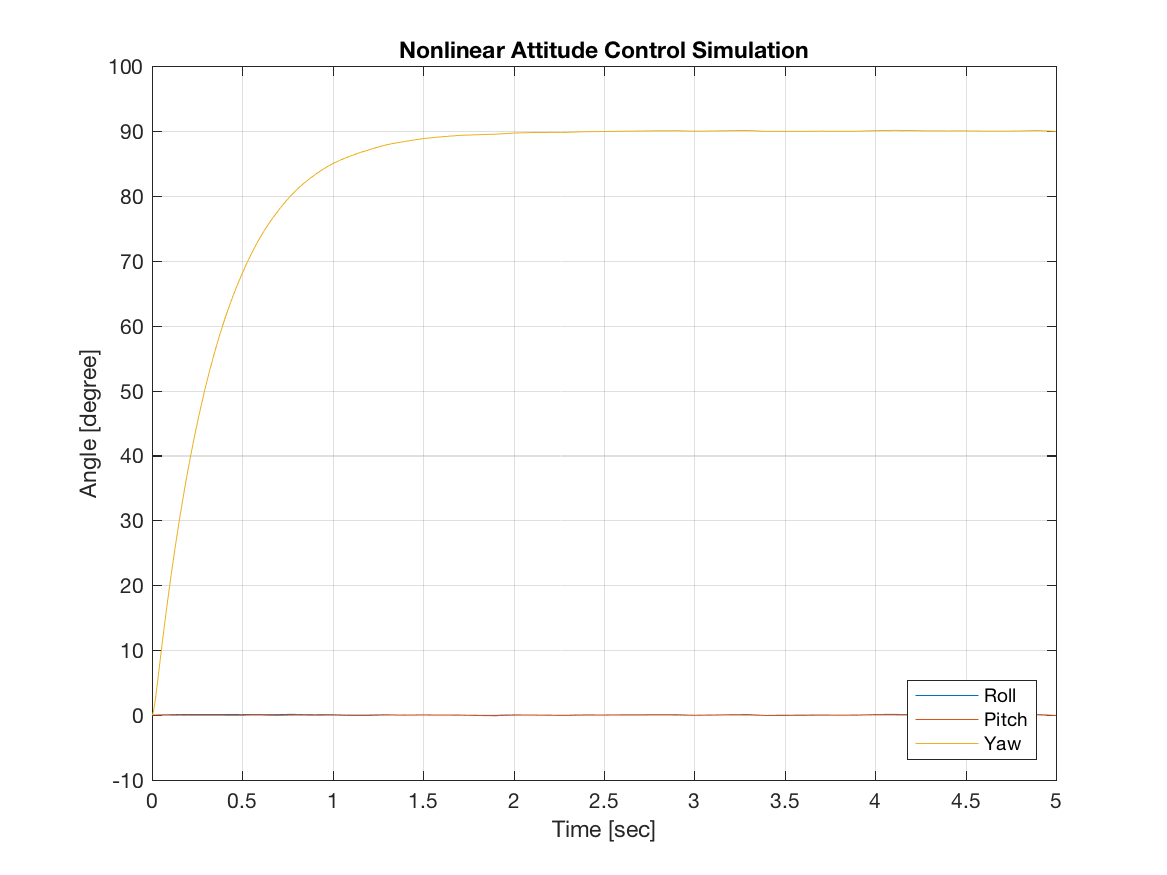
\includegraphics[width=0.45\textwidth]{graphics/yaw_half_non.png}
    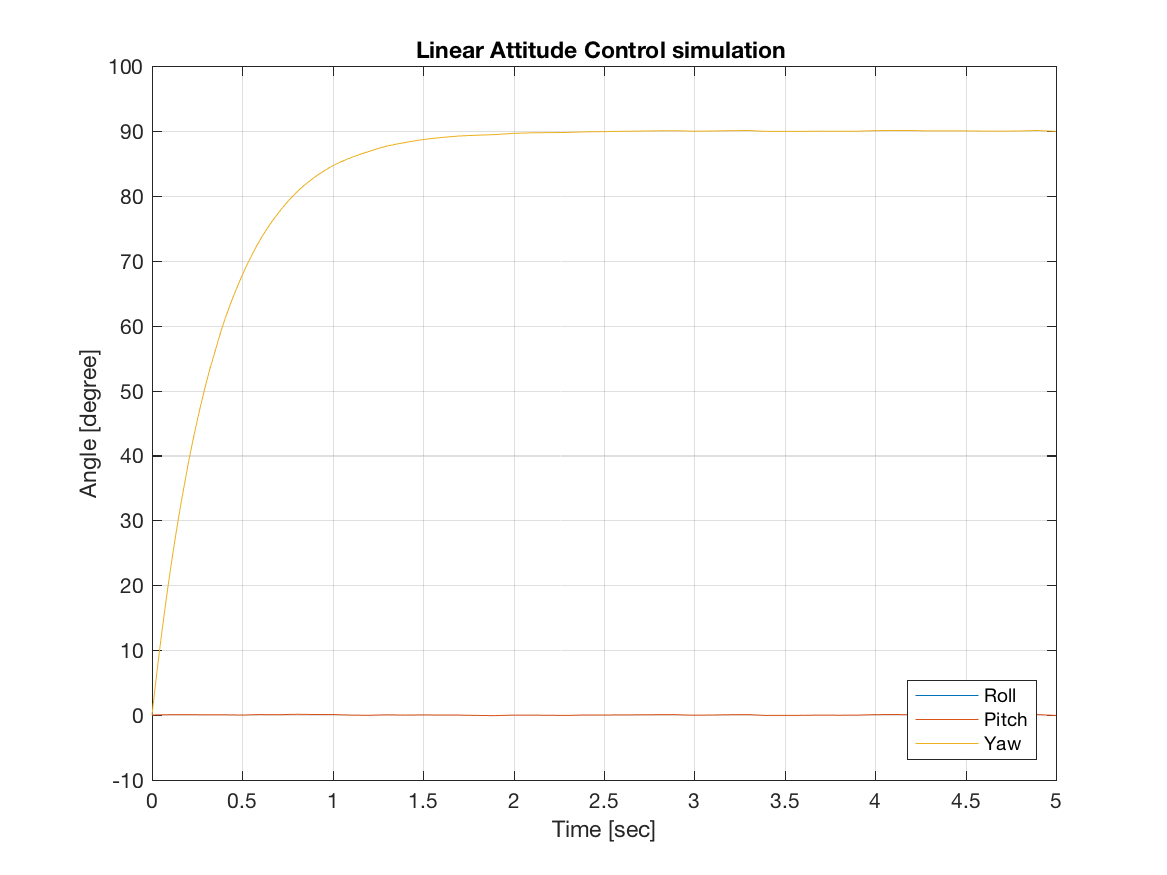
\includegraphics[width=0.45\textwidth]{graphics/yaw_half_pid.png}
    \caption{Simulation Result (Case 6)}
    \label{fig:sim_6}
\end{figure}

\begin{figure}
    \centering
    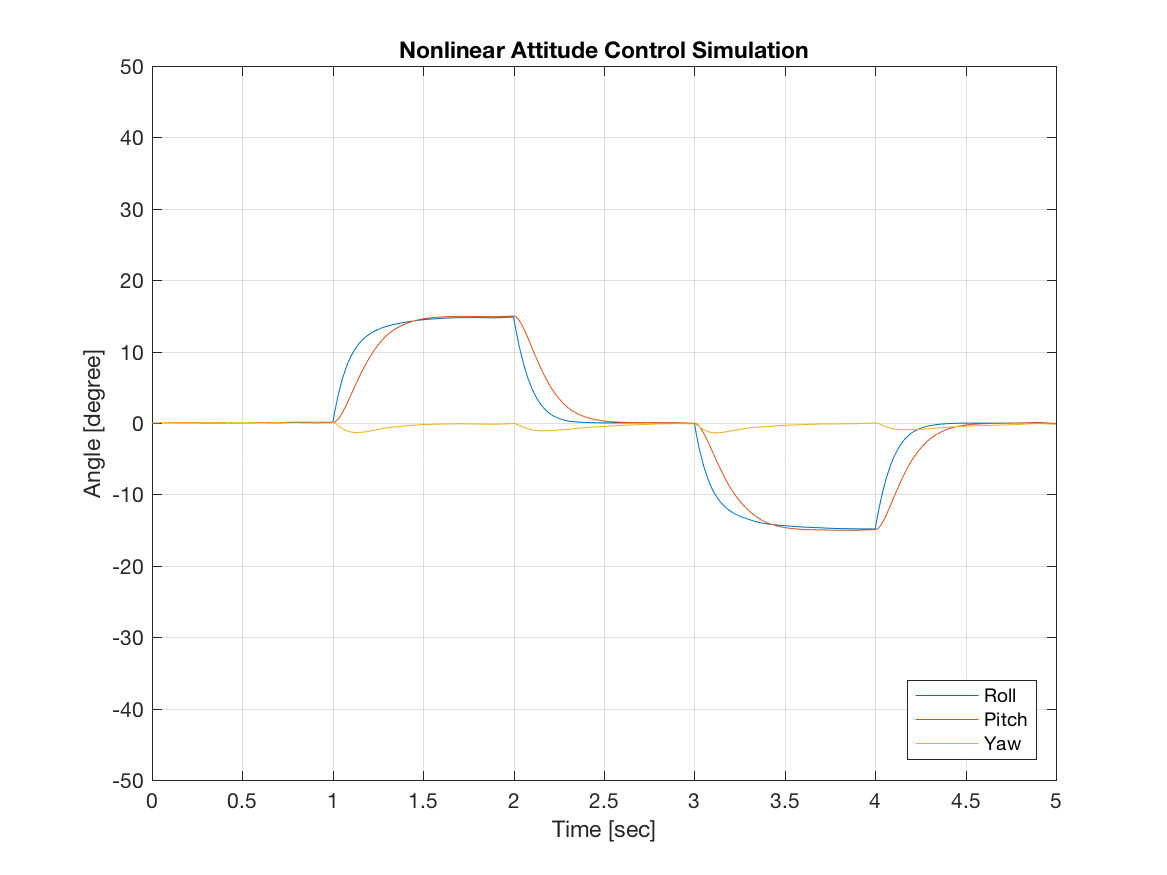
\includegraphics[width=0.45\textwidth]{graphics/custom_01_non.png}
    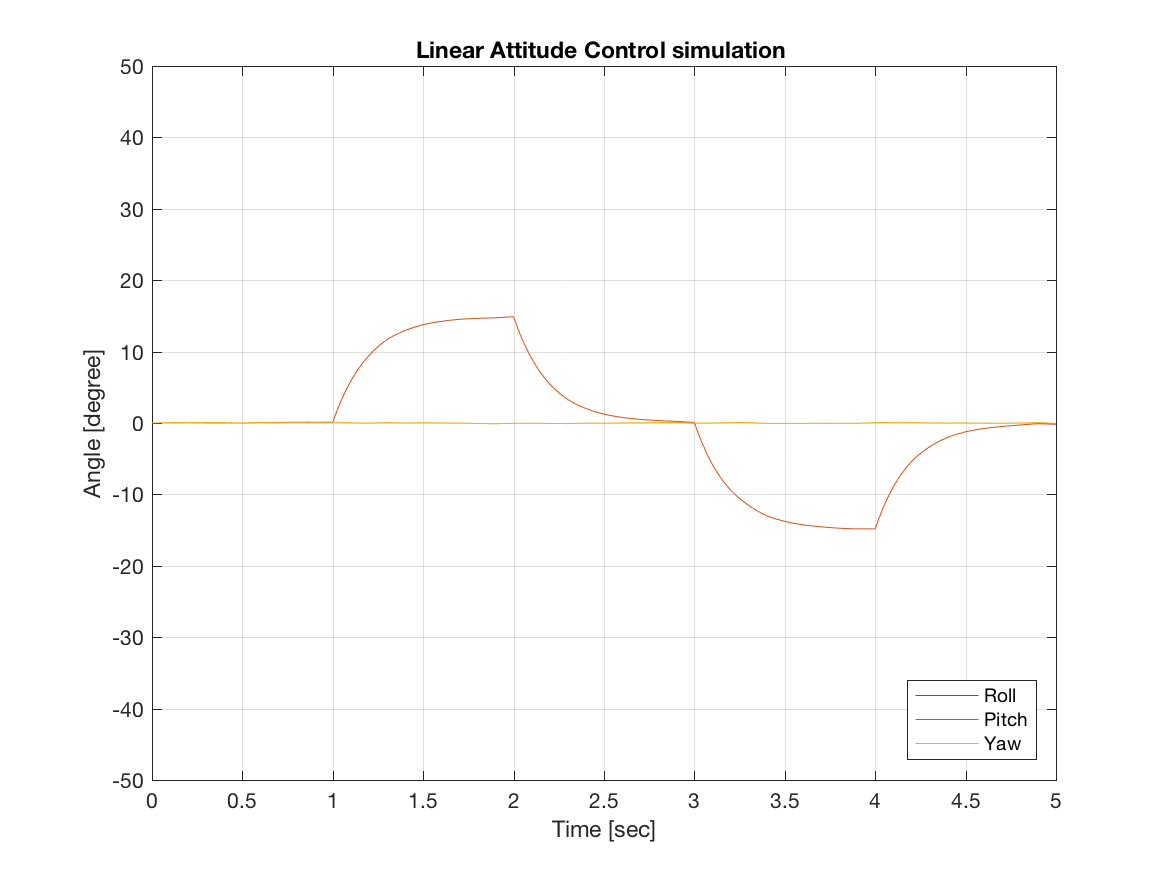
\includegraphics[width=0.45\textwidth]{graphics/custom_01_pid.png}
    \caption{Simulation Result (Case 7)}
    \label{fig:sim_7}
\end{figure}

%%%%%%%%%%%%%%%%%%%%%%%%%%%%%%%%%%%%%%%%%%%%%%%%%%%%%%%%%%%%%%%%%%%%%%%%%%%%%%%%%%%%%%%
\subsection{Discussion}
In most cases, the attitude of the quadrotor converges to the desired attitude faster with the nonlinear control system than it does with the PID linear controller. With roll and pitch changes, the attitude becomes close enough to desired attitude within 0.3 sec at the nonlinear attitude control, and 0.8 sec at the linear attitude control. In the cases of yaw, the rate of convergence is approximately the same for both control systems; the attitude converges to the desired attitude within 1.5 sec. From these results, it can be concluded that the nonlinear attitude controller has the advantage of fast conversion with a guaranteed property robustness \cite{Morgan16}\cite{chung13} . The improvement of the attitude control is expected from global exponential stability of the nonlinear attitude controller. In Figure \ref{fig:sim_7}, the response time of the nonlinear attitude controller is fast enough so that the attitude of the quadrotor stabilize quickly, even with rapid change of desired attitude. Therefore, the nonlinear attitude controller is more suitable for high-agility performance. The deference of response time of the nonlinear attitude control with respect to roll, pitch, and yaw may be caused by the difference of the inertia values along axises, \(I_{xx}\), \(I_{yy}\) and \(I_{zz}\). 

However, the yaw error of the nonlinear attitude control is greater when desired attitude changes in Case 5, than one of the linear attitude control. This is potentially caused by dependency among each angular velocity parameter \(p\), \(q\), and \(r\) at the nonlinear attitude controller. As shown at Equation (\ref{eq:control_law}), each variable cannot be decoupled, while the PID control deals each angular velocity independently. Also, the roll and pitch of the nonlinear attitude controller show different performance, while the the ones of the linear attitude controller are similar to each other. The difference of the inertia among each axis of the body frame possibly causes the asymmetry of the performance.